\title{ARAcalTA part}
%\date{\today}

\documentclass[12pt]{article}
\usepackage{color}
\usepackage{subfigure} 
\usepackage{units}
 \usepackage{graphicx}
\begin{document}

%\maketitle
\subsection{ARAcalTA experiment}
%\paragraph{ARAcalTA experiment}
The ARA experiment \color{red} [cite ARA] \color{black} aims at the measurement of the radio signal produced by high energy neutrino-induced showers in the south pole ice.   
An experiment ARAcalTA was performed using the TA ELS electron beams
to characterize the Askaryan effect and the origin of the radio signal as well as to confirm the detector simulation and calibration \color{red} [cite ARAcalTA].
\color{black}
Therefore, ARAcalTA is primarily designed to observe the coherent emission from an electron shower produced inside an ice block target when the electron beam of the ELS enters into the target. 
The radio signal is collected by the same antennas as the ones used in ARA, they are tuned around a frequency of 300MHz and have a dipole like field of view.
Besides the run operated with the ice target, ARAcalTA  also acquired data of the radio background produced when no target was present, i.e. when the beam was shot directly into the air. 
These data showed a clear radio signal in coincidence with the beam bunches, the sudden appearance signal. 

%\paragraph{Beam setup}
\subsubsection{The experimental setup \color{red}(This section might go into the appendix)\color{black}}
ARAcalTA used the ELS as a source to produce the radio signal almost exactly same as described in the Section  \color{red}III (?). \color{black}
One significant change brought to the ELS setup was the reduction of the bunch length.
The bunch length had been originally set by hardware to a minimum of 20 ns.
The length was decreased by another fast pulser to around 2 ns this time to reduce the destructive
interference at high frequency.
%In this way we prevented destructive interference in the emitted radio signal from early and late part of the shower. 
However such a short pulse, or equivalently such high frequencies, implies to pay a special care to the measurement of the beam monitor signal and especially the modifications in shape and amplitude it can undergo along the transmission in cable.
For the charge measurement, in addition to the Faraday cup and the pickup coil, a Wall Current Monitor was setup to permit the measurement of the charge waveform without absorbing the charge unlike the Faraday cup.
\begin{figure}[!h]
  \centering
  \hspace*{-3ex}
  \subfigure{\includegraphics[width=0.59\linewidth]{ARAcalTAscheme.eps}}
  \caption{Scheme of the ARAcalTA experiment \color{red} (It would be nice to show such schematic plots for all experiments. One with a combined plot showing the location of the experiments.) \color{black}}
  \label{fig:scheme}
\end{figure}

%\paragraph{Detector setup}
The ARAcalTA detector is based on the ARA experiment detector. Two biconical antennas, tuned in the UHF band between 200 and 800MHz, serve as sensors and are of the same design as the ARA vertical polarization antennas. In ARAcalTA they are set up orthogonally to measure two polarizations. Each of them is directly followed by a bandpass filter which selects the frequencies between 230 and  430 MHz to cut the environmental noises at the Utah experimental site, and then a low noise amplifier boosts the signal by a gain of about 40dB.  The signal is transported by low attenuation cable LMR-400 of 40 meters long and recorded with a fast oscilloscope at 10 GSa/s. A simulation of the antenna and a calibration of the electronics components in laboratory were carried out prior to the experiment. 
We also performed a calibration run to verify the detector simulation using a calibrated antenna as a source.
The error on the power measurement from the detector simulation was reduced to less than 15\% \color{red} [cite \ icrc \ reference] \color{black}. 
\\ The experiment was carried out in January 2015, together with the "Brussel experiment". 
%The antennas are placed according the sketch shown in the Figure~\ref{fig:scheme}. 
The configuration of the experiment is shown in the Figure~\ref{fig:scheme}. 
The antennas were located at a perpendicular distance of 7.3 m from the beam axis and their height could be varied. These data allow us to study its angular distribution as well as the sudden appearance signal absolute intensity.

\begin{figure}[!h]
  \centering
  \hspace*{-3ex}
		\subfigure{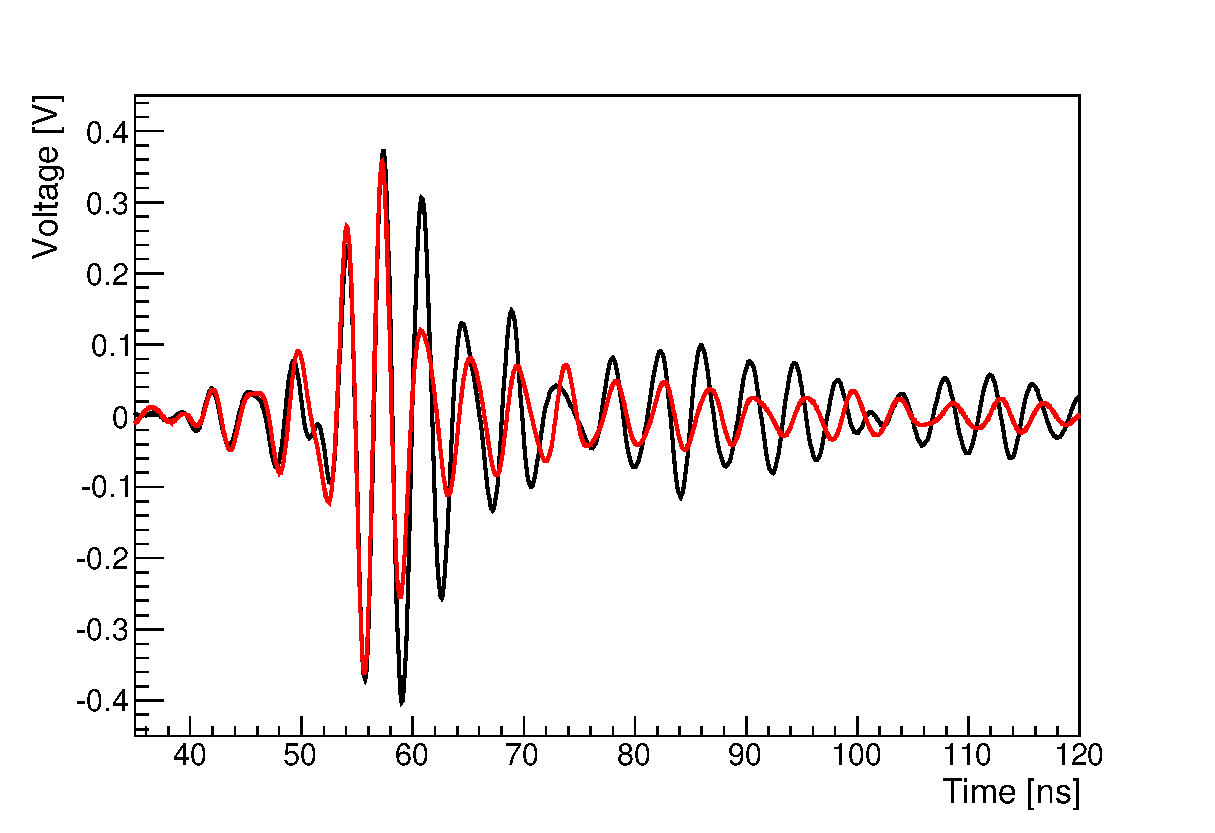
\includegraphics[width=.6\linewidth]{waveformkeiichi}}
  \caption{ \color{red} (Figure need to be updated) \color{black}  Example of a radio waveform recorded with ARAcalTA detector during the run with no ice target.}
  \label{fig:waveform}
\end{figure}

%\paragraph{Data description}
\subsubsection{Data and Resutls}
We collected data without the ice target at 9 different heights ranging from 0 to 7.4 m with respect to the point where the beam exits the container allowing us to probe the sudden appearance intensity at angles from 0$^{\circ}$ to 45$^{\circ}$. A typical radio waveform is shown in the Figure~\ref{fig:waveform}. 
The power is extracted from the averaged waveform after subtracting the pedestal . 
The beam charge signal is recorded with the wall current monitor which was first calibrated with the Faraday cup on a dedicated calibration run. 
The radio signal as a function of the charge is fitted with a power law and the exponent is found to be \color{red} [2.?? +- ?? ]\color{black} indicating pure coherence of the signal as shown in the Figure~\ref{fig:cohe}. 
The polarization of the signal is also almost purely vertical. 
These linear polarization and the quadratic dependence of the signal on the charge are features expected from the sudden appearance signal.

The measured radio intensity with the elevation angle of the antenna is shown in the Figure~\ref{fig:angdist}. The sudden appearance signal is simulated using a realistic charge profile as described in ~\ref{sec:simulation}\color{red} [ cite simulation section ]\color{black}, then
the full detector response is followed.
This includes the convolution of the previously obtained electric field  with a simulated antenna response in the time domain. The obtained voltage is in turn multiplied with the gains of the analogical chain (filter, amplifier and cables). The simulated and measured intensities are consistent with each other.

\begin{figure}[!h]
  \centering
  \hspace*{-3ex}
  	\subfigure{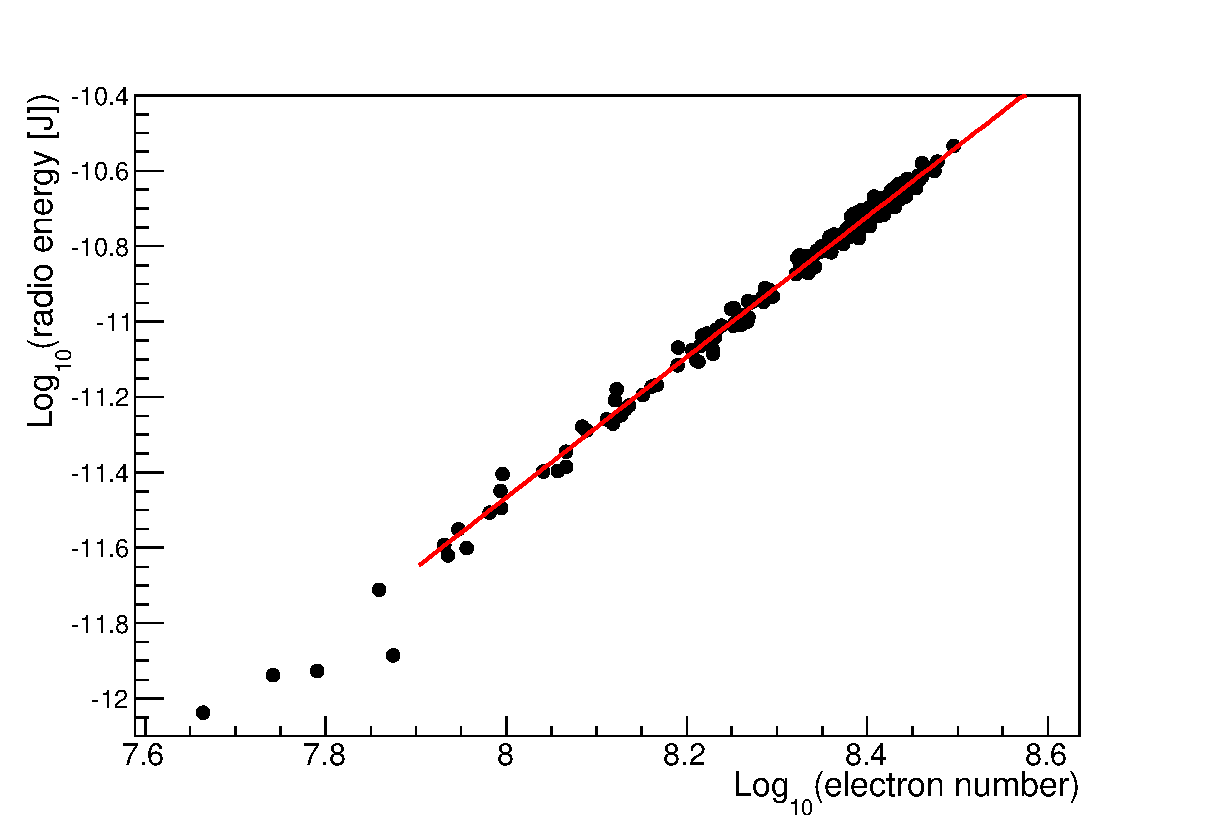
\includegraphics[width=0.7\linewidth]{coherence.eps}}	        
	\caption{ \color{red} (Figure need to be replaced) \color{black} 
	Measured radio emission power as a function of electron number in the beam
	without any target for the antenna elevation angle of 0$^{\circ}$. 
	The slope is 2.??±???, showing a high coherence.	}
  \label{fig:cohe}
\end{figure}

\begin{figure}[!h]
  \centering
  \hspace*{-3ex}
  	\subfigure{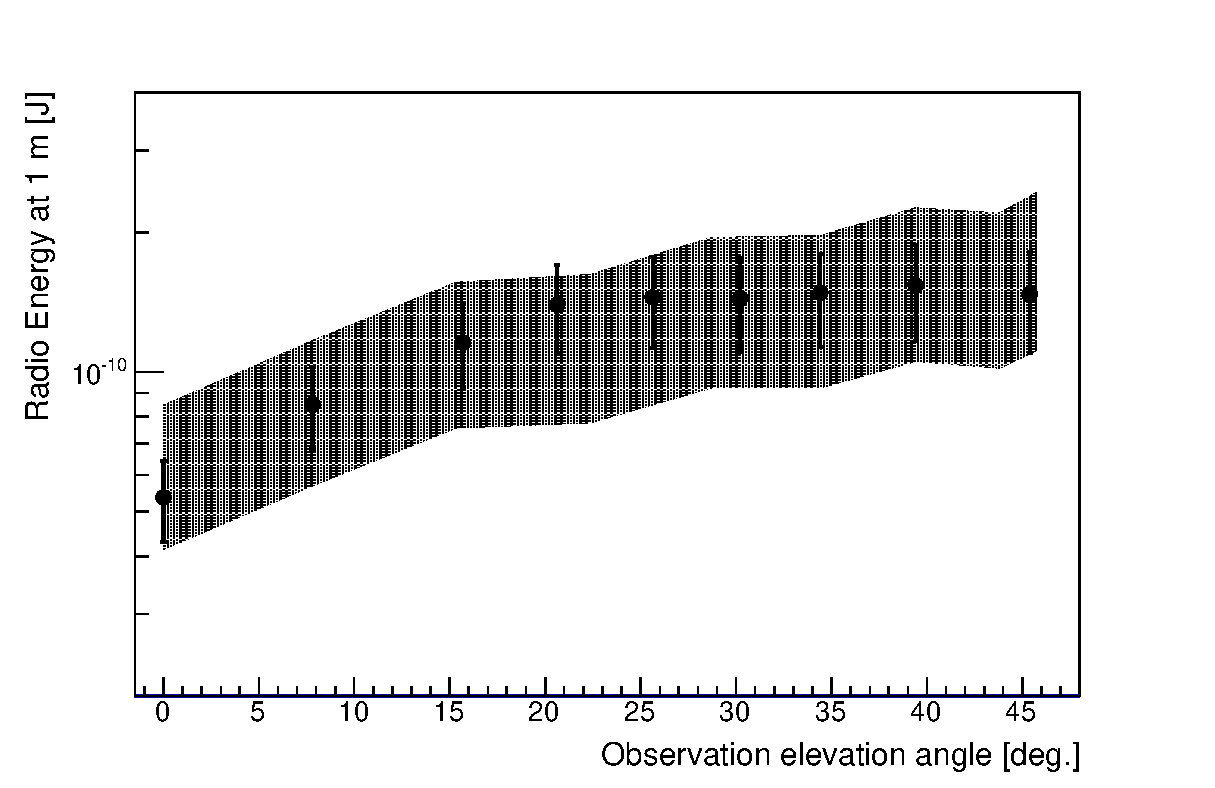
\includegraphics[width=0.7\linewidth]{angulartemporary.eps}}	        
	\caption{ \color{red} (Figure need to be finalized) \color{black} 
	Angular dependence of the sudden appearance radio energy. 
	The energy in this plot is the observed energy before the correction of the detector
	gain as well as the antenna angular response, while the energy is scaled to one at 1 meter
	with a quadratic distance dependence. 
%	The shaded area is the simulation and the error band accounts for \color{red} ??? \color{black}
	The shaded area indicates the simulation with the overall uncertainties (1$\sigma$)
	that accounts for the beam bunch length and measured antenna gain in laboratory.
	}
  \label{fig:angdist}
\end{figure}

\end{document}
